\documentclass[journal]{IEEEtran}
\usepackage{amsmath}
\usepackage{mathptm}
\usepackage{url}
\usepackage{times}
\usepackage{graphicx,color}
\usepackage{CJKutf8}
\usepackage{multirow}
\usepackage[labelformat=simple]{subcaption}
\renewcommand\thesubfigure{(\alph{subfigure})}

\begin{document}
\title{SmartPatch: A Self-Powered and Patchable Cumulative UV Irradiance Meter}

\author{
	Donkyu~Baek,~\IEEEmembership{Member,~IEEE,}
	Hyung~Gyu~Lee,~\IEEEmembership{Member,~IEEE,}
	and~Naehyuck~Chang,~\IEEEmembership{Fellow,~IEEE}

%\thanks{}
\thanks{Direct questions and comments about this article to Naehyuck Chang, Korea Advanced Institute of Science and Technology, 291, Daehak-ro, Yuseong-gu, Daejeon, Korea (e-mail: naehyuck@cad4x.kaist.ac.kr.) This work was supported by the Center for Integrated Smart Sensors funded by the Ministry of Science, ICT \& Future Planning as Global Frontier Project (CISS-2015M3A6A6066117) and the National Research Foundation of Korea(NRF) grant funded by the Korea government(MSIP) (No. 2015R1A2A1A09005694.)}
}

% make the title area
\maketitle

\begin{abstract}
\textcolor{red}{Ultraviolet (UV) irradiance affects human bodies both positively and negatively. We introduce SmartPatch, a self-powered, small-form-factor, light-weight, low-cost, and a patch-type UV meter, that provides a scientific measure of UV radiation and irradiation on a particular skin area. It is powered by a tiny PV (photovoltaic) cell without a battery and a power converter and performs UI (user interface) without a physical switch.} 
\end{abstract}

% Note that keywords are not normally used for peerreview papers.
%\begin{IEEEkeywords}
%Ultraviolet, skin damage, UV irradiance meter, dynamic power management.
%\end{IEEEkeywords}

%%%%%%%%%%%%%%%%%%%%%%%%%%%%%%%%
%% START%%%%%%%%%%%%%%%%%%%%%%%%%%
%%%%%%%%%%%%%%%%%%%%%%%%%%%%%%%%

%%%%%%%%%%%%%%%%%%%%%%%%%%%%%%%%
\section{Introduction}
%%%%%%%%%%%%%%%%%%%%%%%%%%%%%%%%

\textcolor{red}{A proper level of ultraviolet (UV) \textit{irradiation (time integral of irradiance\footnote{The radiant of UV energy per area.})} on the human skin is essential as it stimulates synthesis of Vitamin D. Human skins can endure a certain level of UV irradiation, but over-irradiation may cause skin damage and can even develop a fatal disease.}
Therefore, modern society humans are generally warned to avoid excessive UV irradiation even during their daily life.

\textcolor{red}{The intensity of UV irradiance is often quantified by the UV index (UVI). Region-based daily UVIs are commonly broadcasted through weather forecast channels. There are general guidelines to avoid skin damage classified with the UVI as shown in Fig.~\ref{fig:guidelines}. For example, we are recommended to stay indoor when the UVI  is over 8.} 

\textcolor{red}{In order to safely perform outdoor activities without experiencing skin damage, we should be aware of  the maximum UV irradiation. UVI and UV exposure time are easy metrics to estimate UV irradiation for normal people when a medical-grade scientific measure is not accessible. Although we commonly estimate the UV irradiation by the UV exposure time, it cannot be a reasonable estimation of UV irradiation on a particular skin area because UV irradiation is determined by the time integral of the instantaneous UVI accounting the angle between the Sun, in addition to the individual factors such as skin color. Additional UV protection such as sunscreen lotion makes it even more difficult.} 

\textcolor{red}{It is crucial to directly measure the UV irradiance and irradiation on the target skin surface of interest, \textit{i.e.} a UV sensor must be directly mounted on the skin surface of interest with the same angle to the Sun. The UV meter continuously reads the UV sensor and integrates the value over time. Unfortunately, to the best of our knowledge, existing UV measuring tools for normal people (excluding a laboratory measurement setup) can hardly achieve this goal.}

\begin{figure}
\centering
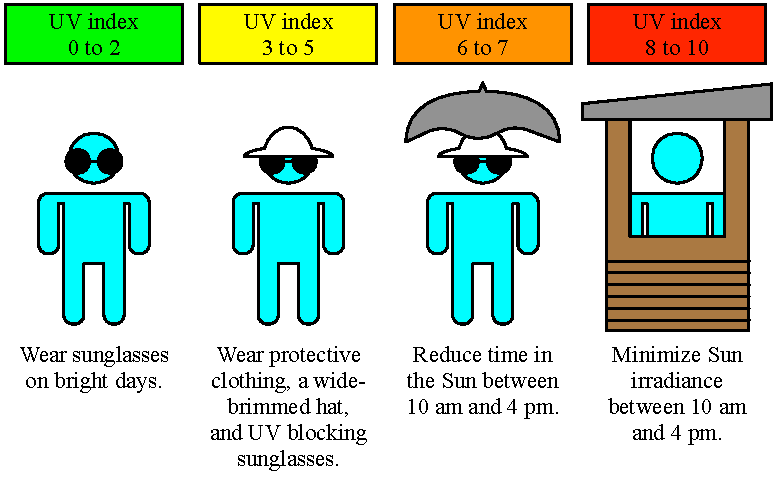
\includegraphics[width=1.0\hsize]{Figures/UVI_guideline.pdf}
\caption{Guidelines to protect oneself from overexposure to UV irradiance (US Environmental Protection Agency.)}
\label{fig:guidelines}
\end{figure}

\textcolor{red}{In this article, we introduce SmartPatch, a solar-powered and patchable smart UV irradiation meter that informs both the current UV irradiance and irradiation. SmartPatch is designed to attach on the skin surface of interest, its UV measurement meets the above mentioned requirements such as the angle to the Sun, environmental change and body movement. Two key technologies are behind the proposed SmartPatch. The first is a storage-less and converter-less energy harvesting~\cite{Lee:ASPDAC15} that does not require a battery nor a voltage converter for solar energy harvesting. The second is a switch-less user interface. These two technologies can significantly reduce both volumetric and gravimetric overheads as well as the manufacturing cost.}

\textcolor{red}{SmartPatch detects the correlation between the UV irradiance and solar irradiance. Natural operation keeps a high correlation between them. The correlation is broken if the UV sensor is intentionally blocked by a finger. SmartPatch detects such finger actions and utilizes them for UI (user interface) as if physical switches are pressed by the finger. A smartphone LED flashlight can do the same job. We design an app that  generates pre-defined light flashing patterns so that a single screen touch can replace multiple times of finger actions. These technologies make it possible to implement SmartPatch with simple integrated circuits in a single chip, and also make it possible for a tiny PV cell to directly supply power to the chip without a power converter and a battery. As a result, SmartPatch becomes extremely low-cost, low profile, small, and light.}

 \textcolor{red}{The main functions of SmartPatch include 1) displaying the current UVI, 2) displaying the remaining UV irradiation to avoid skin damage, and 3) mode change or parameter setting for the personalized skin type and the SPF (Sun protection factor) of the currently applied sunscreen lotion. We verified the functionalities and usefulness of SmartPatch performing various outdoor activities.}

\section{Backgrounds}

\subsection{Basics of UV and Skin Damage}

Among overall range of UV radiation emitted toward the Earth, only UVA (320 to 400 nm) and UVB (280 to 320 nm) penetrate the atmosphere and affect humans and environment. UVA causes skin aging and wrinkle while UVB causes well-known skin damage such as erythema (redness of the skin), sunburn and skin cancer~\cite{Matsumura:TAP04}.

\textcolor{red}{Human skin has an ability to protect itself from the UV irradiation by skin darkening and thickening. When the skin absorbs UV irradiance, It produces a dark-coloured pigment (called melanin) that delays the skin damage from two to four times. The degree of darkening effects is different by the skin types~\cite{Harrison:Method02}.}

\textcolor{red}{Even though skin damage is caused by the UV irradiation instead of the current UV irradiance, we first have to quantify UV irradiance as  a standard metric to quantify the impact of UV irradiation to the human skin.}
Minimal erythema dose (MED), which is widely used to assess skin sensitivity to the UV irradiation, is defined as the lowest UV irradiation that produces minimally perceptible erythema~\cite{Diffey:CPPM91}. The relative effectiveness for the MED by the wavelength of UV radiation is defined and introduced by the International Commission on Illumination~\cite{CIE}. Erythema effectiveness by the UVB is 10 to 100 times larger than the effectiveness by the UVA. The Sun spectrum multiplied by the erythemal effectiveness is the effective UV spectrum, and a result integrated over the whole spectrum is the effective UV irradiance and used as a measure of the UV irradiance.
\begin{equation}
\text{Effective~UV~irradiance} = \int A(\lambda)E(\lambda) d \lambda
 \end{equation}
where \textcolor{red}{$\lambda$ is the wavelength}, $A(\lambda)$ is the Sun spectrum, and $E(\lambda)$ is the erythemal effectiveness by the wavelength. \textcolor{red}{Finally, UVI is obtained dividing (1) by 0.025 $mW/m^2$~\cite{CIE}.}
\begin{equation}
\text{UVI}= \frac{\text{Effective~UV~irradiance}}{0.025~mW/m^2.}
 \end{equation}

We use sunscreens to protect our skin from UVB irradiance. Sun protection factor (SPF) is defined by \textcolor{red}{the fraction of sunburn-producing UV that reach the skin} calculating as a following equation,
\begin{equation}
\text{SPF} = \frac{\int A(\lambda)E(\lambda) d \lambda}{\int A(\lambda)E(\lambda) / \text{MPF}(\lambda) d \lambda}
 \end{equation}
where MPF means monochromatic protection factor.

A bigger number of SPF \textcolor{red}{implies a higher reduction rate} of UV absorption and \textcolor{red}{efficiently} reduces chances of skin damage. For example, a sunscreen with SPF 15 blocks 93\% of UV irradiance and extends the time to produce erythema about 15 times longer. \textcolor{red}{Such a high rate of UV filtering certainly extends UV exposure time without skin damage, UV irradiance is still accumulated in the skin even with a sunscreen regardless of the SPF, and it may eventually incur skin damage.}

\textcolor{red}{Finally, the maximum allowable UV exposure time is calculated by a function of skin type, instantaneous UVI and the SPF of a sunscreen.} 
\begin{equation} \label{eq: max_exp_time}
\begin{split}
\text{\rm Maximum~UV~exposure~time}
&= \frac{\rm Maximum~UV~irradiation}{\rm Effective~UV~irradiance} \\
&= \frac{\text{MED}(\text{skin~type})}{\int A(\lambda)E(\lambda)  / \text{MPF}(\lambda) d \lambda} \\
&\approx \frac{\text{MED}(\text{skin~type})\times \text{SPF}}{\text{UVI} \times 0.025~mW/m^2}.
\end{split}
\end{equation}


\subsection{UV Meters}
\textcolor{red}{There are various portable UV meters on the market as shown in Fig.~\ref{fig:UVI_meters}(a). Most UV meters can only measure the instantaneous UVI though we emphasize UV irradiation measurement is meaningful. Some top-of-the-line UV meters (Fig.~\ref{fig:UVI_meters}(b)) additionally inform UV irradiation. They are capable of notifying the maximum allowable UV exposure time based on the instantaneous UVI, skin type and SPF. In other words, the feature basically meets the requirement.  First, however, these devices typically include a battery~\cite{Netatmo, Ultra}. The types of such class devices are often a wrist strap, a watch, a pendant, or a badge. So, second, such devices can only measure the UV irradiance of limited positions of the human body, which is unlikely vulnerable to sunburn.} 
%
As shown in Fig.~\ref{fig:UV_exposure_skin}, each skin surface area has a distinctly different amount of UV irradiance due to the different angle to the Sun. In addition, partial shading can continuously occur on each skin surface area by trees, buildings, other body parts, clothes, and so forth. For instance, people often experience skin damages on their shoulders while other skin areas (\textit{e.g.}, a wrist that has the UV strap) are manageable even if the whole body has been exposed to the Sun.

\begin{figure}
\centering
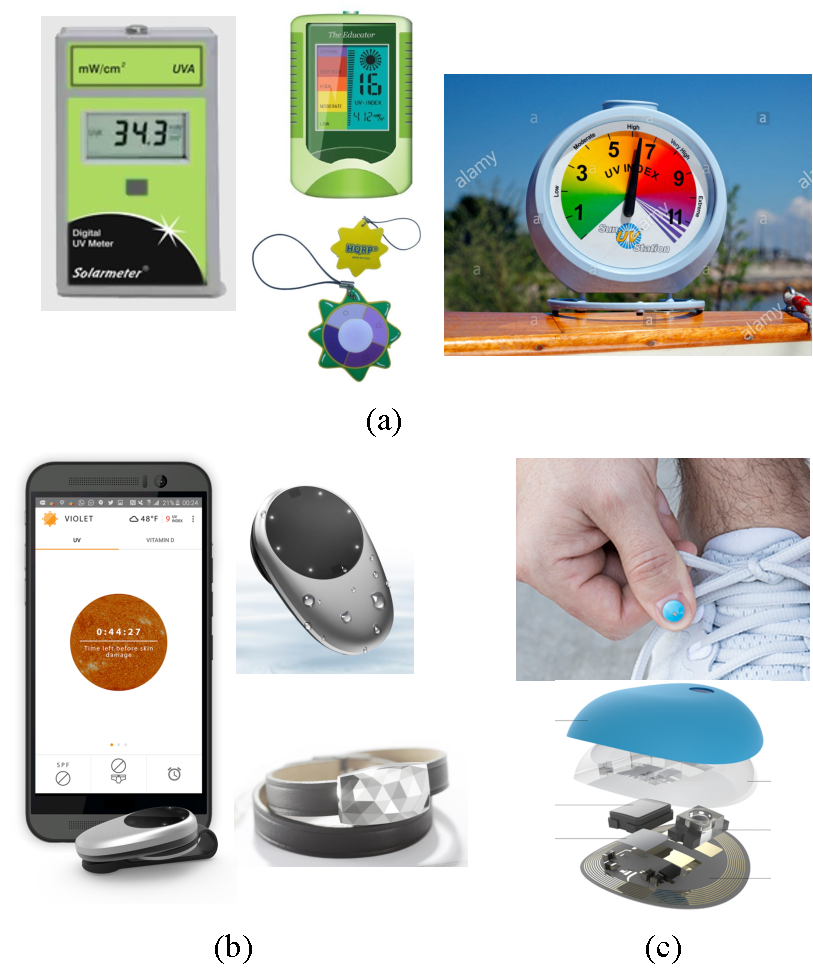
\includegraphics[width=0.8\hsize]{Figures/UVI_meter.pdf}
%\caption{(a) Simple UV irradiance meters that inform the instantaneous UV irradiance level only and (b)--(c) advanced UV irradiance meters that calculate the maximum UV exposure time based on the skin type and the SPF of the sunscreen~\cite{Netatmo, Ultra, LOreal}.}
\caption{Commercial UV irradiance meters~\cite{Netatmo, Ultra, LOreal}.}
\label{fig:UVI_meters}
\end{figure}

\begin{figure}
\centering
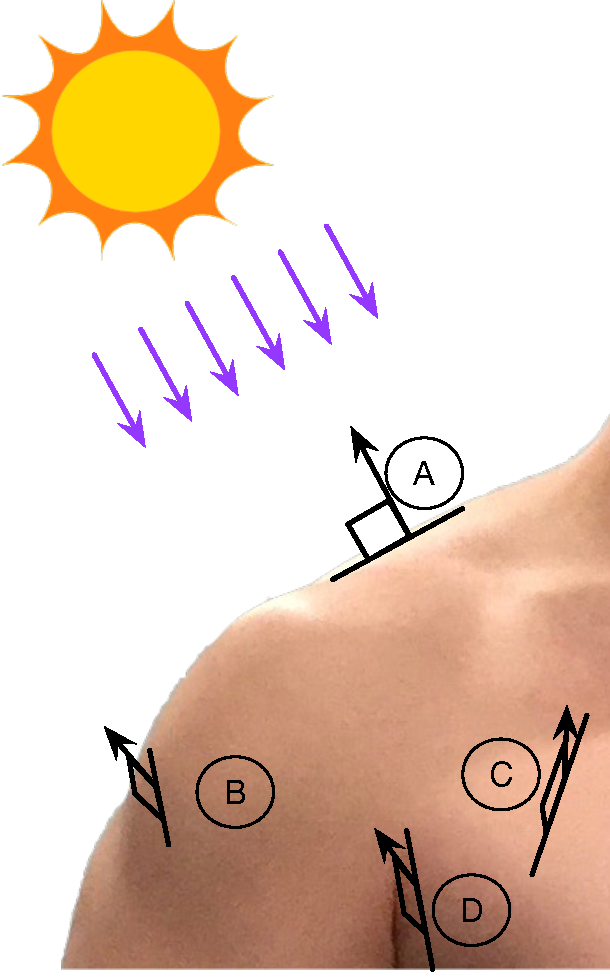
\includegraphics[width=0.4\hsize]{Figures/UV_skin_areas.pdf}
\caption{UV irradiance by the skin areas.}
\label{fig:UV_exposure_skin}
\end{figure}

\textcolor{red}{Therefore, an accurate UV irradiation meter should position the UV sensor on the exact location of the target skin surface with the same perpendicular angle to the Sun. However, it is not practical to mount a separate UV sensor from the \textcolor{red}{UV meter main unit in Figs.~\ref{fig:UVI_meters}(a) and~\ref{fig:UVI_meters}(b)}. Therefore, a patchable design of a UV irradiance meter is only capable of measuring correct UVI. We easily figure out the most vulnerable skin area and attach the device onto it taking into account the environment, our outfit and activities. Recently, a patchable UV meter has been introduced by a cosmetic company as shown in Fig.~\ref{fig:UVI_meters}(c)~\cite{LOreal}. It is powered by the user's smartphone via Near Field Communication (NFC.) However, the device should equipped with a large-size energy storage such as a supercapacitor and thus a power converter to continuously measure the UV irradiation after it has received energy from NFC.}

%%%%%%%%%%%%%%%%%%%%%%%%%%%%%%%%
\section{SmartPatch}
%%%%%%%%%%%%%%%%%%%%%%%%%%%%%%%%

\textcolor{red}{Implementation of a patchable UV irradiation meter is challenging due to the volumetric and gravimetric constraints. A low-profile design is a must as well. Use of a battery is a common solution for the existing UV irradiation meters, but this method eventually ends of with a higher cost, a larger form factor and a heavy weight. We describe the requirement of SmartPatch as follows:}

\begin{itemize}
%\item Covering both the UVA and UVB spectrum,
\item Having a small form factor and possibly disposable,
\item \textcolor{red}{Programming the sunscreen SPF and user's skin type,}
\item Calculating the maximum UV exposure time based on the UV irradiance and skin type,
\item A patchable design to measure the actual cumulative UV irradiance on the exact skin area of interest,
\item Self-powered by a PV cell with the minimum possible size, and
\item No use of a power converter nor significant energy storage.
\end{itemize}

\subsection{Storage-less and converter-less Energy Harvesting Technology}
Most energy harvesting systems adopt energy storage elements as well as power converters, which have been considered as must-have components for performing the maximum power point tracking (MPPT). However, those components seriously limit the design in many aspects such as the weight, form factor, cost, maintainability, etc. Recently, a breakthrough MPPT method that does not require power converters and energy storage elements has been introduced for high-efficiency PV energy harvesting applications~\cite{Wang:ASPDAC14}.

The basic principle of the storage-less and converter-less energy harvesting is to supply the harvested energy from the PV cell directly to the target device using a fine-grained DPM technique. %as shown in Fig.~\ref{fig:architectures}(b). 
Power converter can be simply removed if the voltage level directly supplied from the PV cell is in the range of the operating voltage for the target device. 
%In general, the MPP voltage of the PV cell is maintained within a quite narrow range regardless of the solar irradiance.This implies that the PV cell generates almost-constant voltage output, that is a main role of power converters, as long as we keep the track of the MPP current. 
Fast enough (or fine-grained) DPM makes the PV cell keep the MPP as if the current of the target device is a DC current as long as the average current is the same to the MPP current~\cite{Wang:ASPDAC14}. However, fast DPM may bring non-negligible energy and time overhead during the power state change, and finally the overall energy efficiency is degraded. So a proper control method of the DPM considering the energy overhead is required for enlarging the energy efficiency. We adopt a pulse width modulation (PWM) based DPM in designing of SmartPatch~\cite{Lee:ASPDAC15}. The PWM based DPM controls the duty rate of power-on state compared with power-off state to keep the MPP. This DPM achieves higher energy efficiency as well as the low implementation cost at the same time among various DPM architectures.

DPM is no longer available if the solar irradiance becomes too low, and SmartPatch should be completely shut down. The power management unit (PMU) detects power interruption and allows the non-volatile RAM (NVRAM) to store the necessary context \cite{Balsamo:TCAD16}. NVRAM is solely powered by the small size capacitor while it saves the context, and thus the proposed storage-less and converter-less MPPT allows to save only a very small capacity of context. Fortunately, SmartPatch needs to save just few bytes of information to the NVRAM.

%\begin{figure}
%\centering
%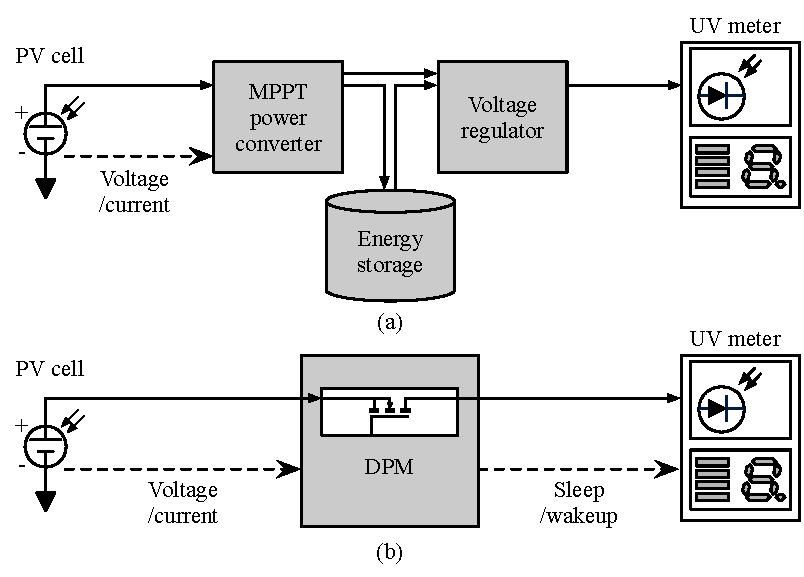
\includegraphics[width=1.0\hsize]{Figures/architectures.pdf}
%\caption{(a) A typical architecture of an energy harvesting system and (b) a storage- and converter-less energy harvesting system~\cite{Wang:ASPDAC14}.}
%\label{fig:architectures}
%\end{figure}
%
%A storage-less energy harvesting architecture raises relatively less technical challenges compared with the converter-less architecture. Instead, it may limit the area of the applications because the target devices become unavailable if the device is lack of harvested energy.
%However, SmartPatch is one of the ideal applications of storage-less energy harvesting because it does not have to measure the UV irradiance when there is no sunlight.

\subsection{A switch-less user interface}
%\textbf{A switch-less user interface enables a low-cost disposable design and an extreme low-profile design.}
A switch (or button) is a necessary component for providing a function control to the users in most devices. However, including a switch in a tiny device largely diminishes the advantages of a small, patchable and a very low-profile design. These three requirements make the switch operation inconvenient and impose a serious design restriction. We develop a switch-less user interface by detecting user generated unique patterns of the UV level change, which cannot be observed in the natural environmental change to the UV sensor and PV cell.

\begin{figure}
\centering
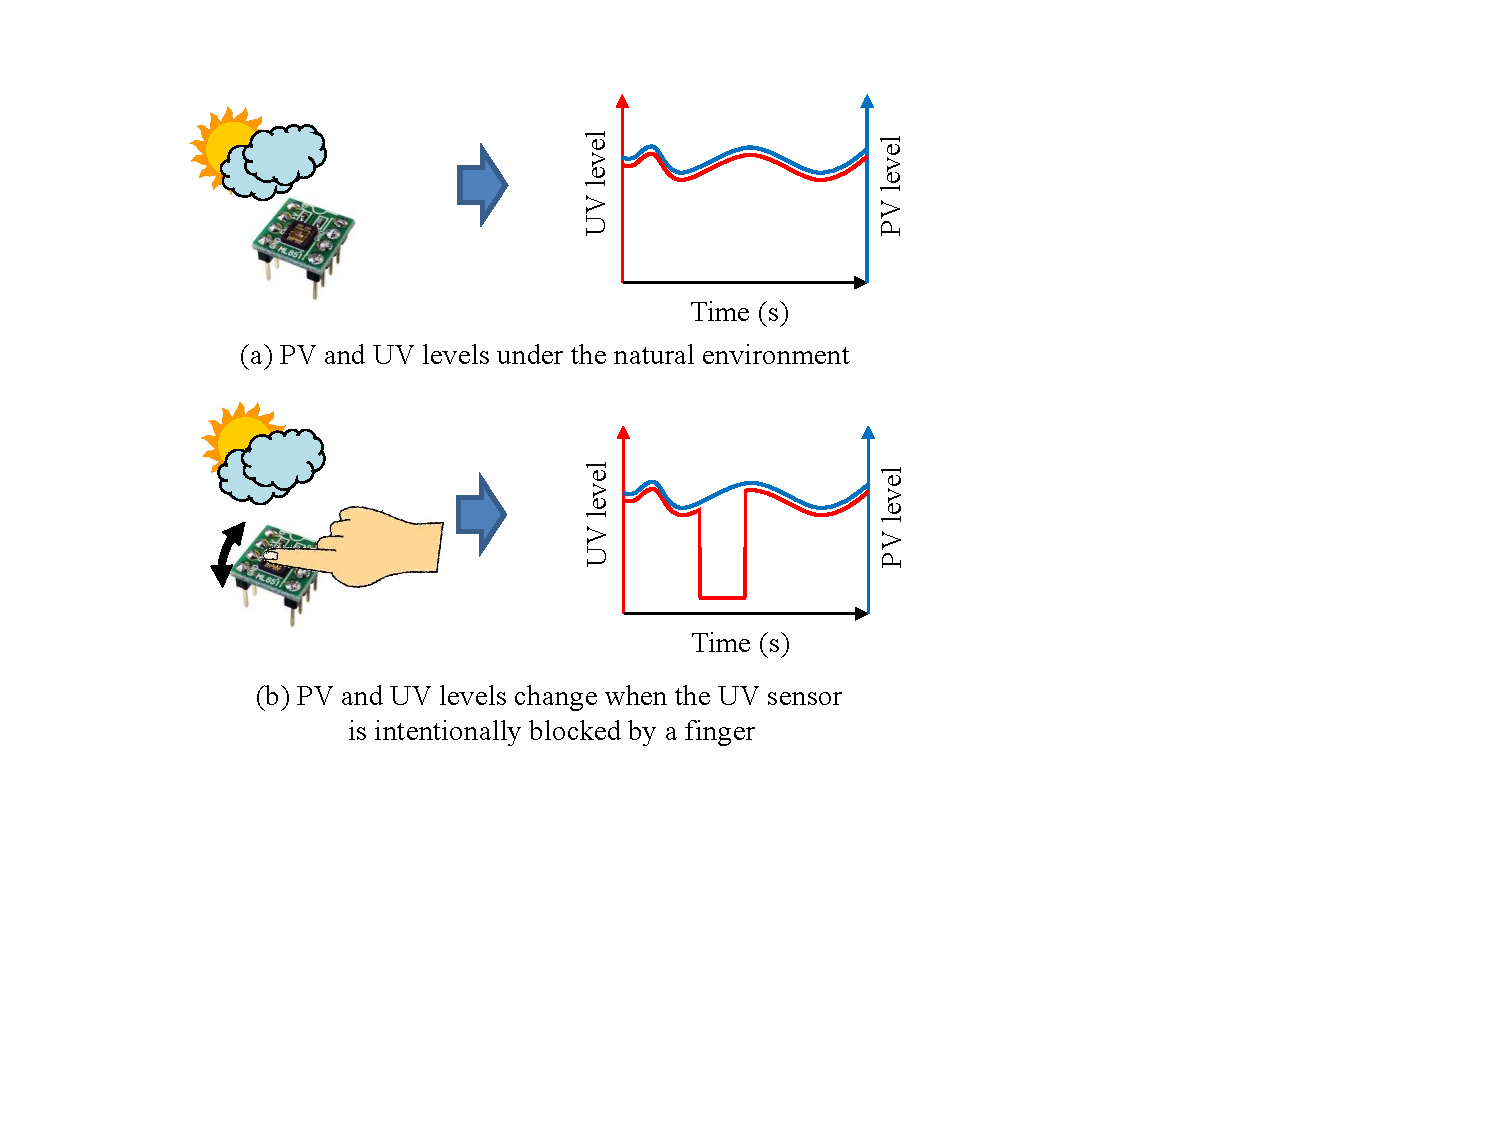
\includegraphics[width=0.8\hsize]{Figures/switchless_interface.pdf}
\caption{Principle of the switch-less interface.}
\label{fig:switchless_interface}
\end{figure}

Fig.~\ref{fig:switchless_interface} shows the principle of the operation of the proposed switch-less user interface. A natural environmental change always makes both the UV level and PV level and they are highly correlated as shown in Fig.~\ref{fig:switchless_interface}(a). The switch-less user interface action requires simple finger actions to block the UV sensor under a good amount of Sunlight. This makes the UV sensor output level is abruptly decreased as shown in Fig.~\ref{fig:switchless_interface}(b) while the PV cell generates enough power to operate SmartPatch. This action is perceived as if there is a virtual switch and pressed by a finger. A sequence and duration of the block and unblock actions of the UV sensor generate specific patterns. A number of unique patterns perform various user interface functions such as skin type setting, resetting the device, etc. \textcolor{red}{We also provide a smartphone app that automatically generate a sequence of LED light flashing actions. User can just touch the  menu buttons (skin type, reset, etc.) of the app,  which replaces the sequence of finger actions.}

\subsection{SmartPatch design}

We design a prototype of SmartPatch using two key technologies mentioned above.
Fig.~\ref{fig:block_diagram} shows a block diagram of the SmartPatch prototype consisting of a PV cell, a PMU, control logic, an NVRAM, a UV sensor, a display, and other glue logic. We implement the PMU with a PWM based DPM architecture. The control logic includes a switch-less user interface. The NVRAM stores the result of the UV irradiance accumulation, user skin type and use of a sunscreen. The display is customized to show the current UV irradiance level as well as the remaining UV exposure time before experiencing skin damages.

%\begin{figure}
%\centering
%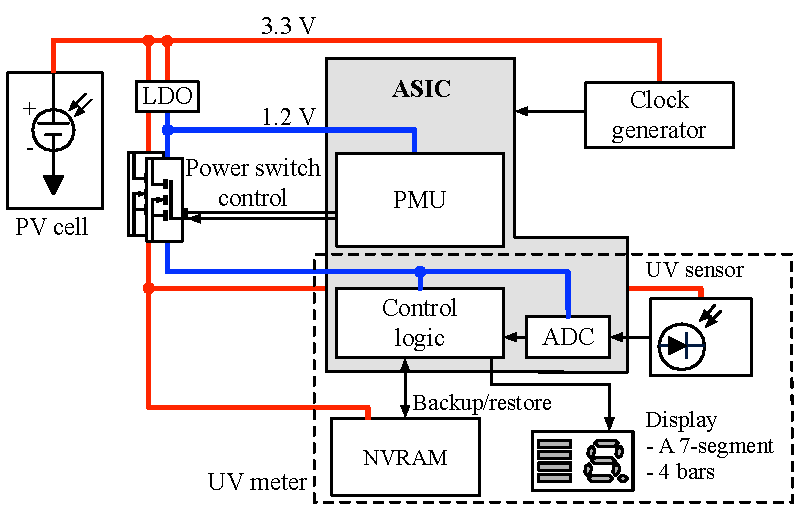
\includegraphics[width=1.0\hsize]{Figures/block_diagram.pdf}
%\caption{A block diagram of SmartPatch.}
%\label{fig:block_diagram}
%\end{figure}
%
%\begin{figure}
%\centering
%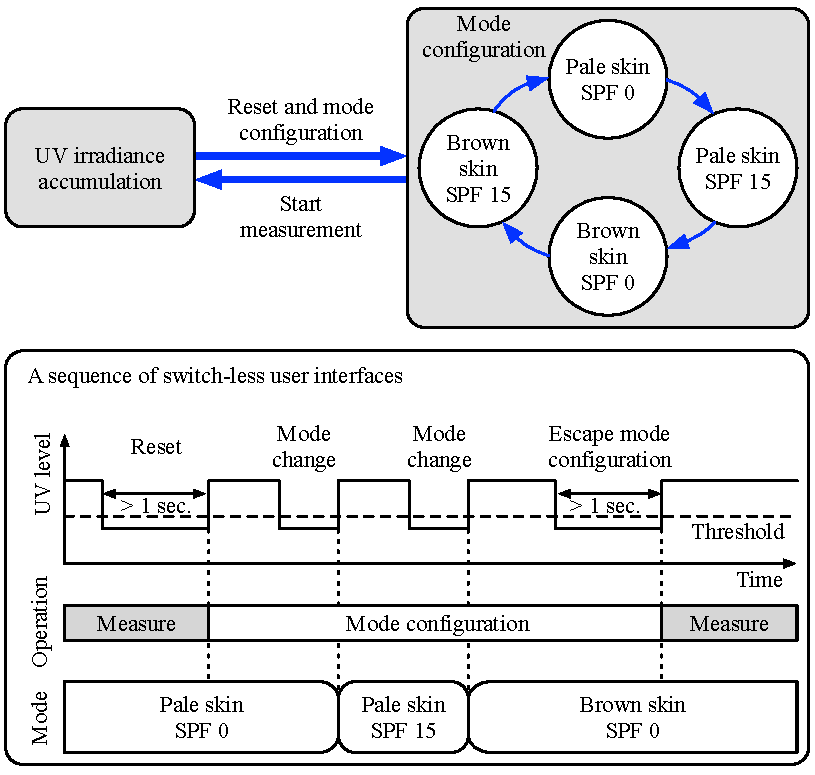
\includegraphics[width=1.0\hsize]{Figures/configuration.pdf}
%\caption{Reset and mode configurations of SmartPatch.}
%\label{fig:configuration}
%\end{figure}

\begin{figure}
\centering
	\begin{subfigure}{0.45\textwidth}
	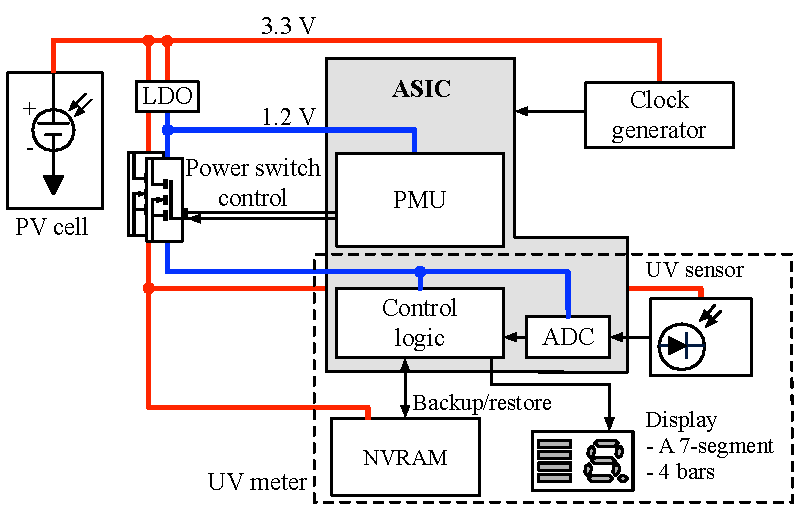
\includegraphics[width=1.0\hsize]{Figures/block_diagram.pdf}
	\caption{}
	\label{fig:block_diagram}
	\end{subfigure}
~
	\begin{subfigure}{0.45\textwidth}
	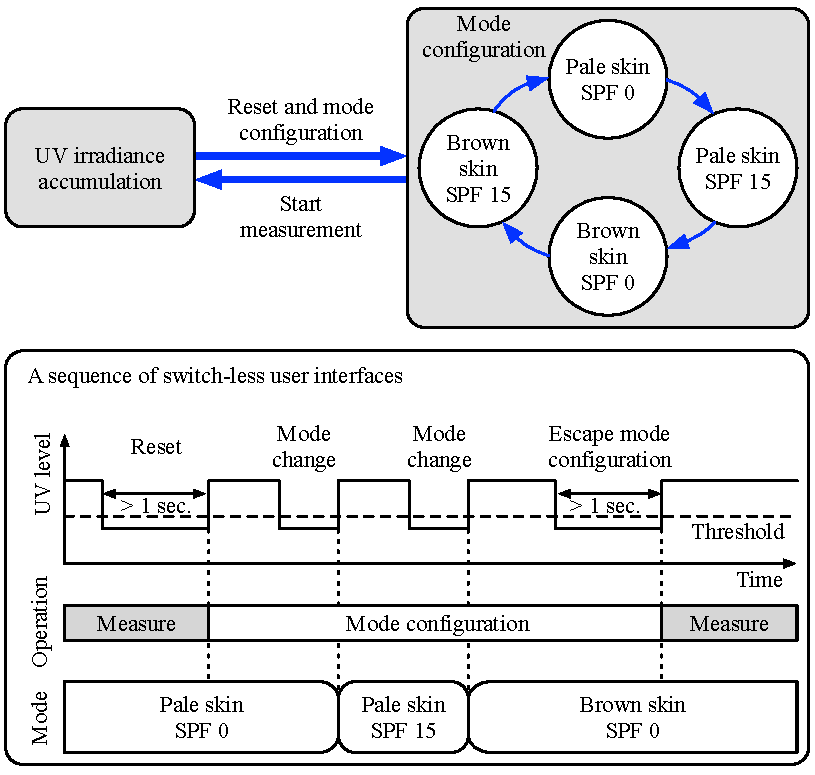
\includegraphics[width=1.0\hsize]{Figures/configuration.pdf}
	\caption{}
	\label{fig:configuration}
	\end{subfigure}
\caption{(a) A block diagram and (b) mode change and parameter setting of SmartPatch.}
\end{figure}

%The current version of SmartPatch embeds two user interface functions: device reset and operation mode change. Adding new features does not incur major design change. Fig.~\ref{fig:configuration} shows examples of the switch-less user interface functions. Blocking the UV sensor for more than a second resets SmartPatch and starts a new mode configuration. \textcolor{red}{The user is supposed to repeat blocking the UV sensor until the desired  mode is set. In Figure~\ref{fig:configuration}, the number of operating modes is designed as four for the demonstration purpose, but it is easily expanded by the use of NVRAM. Repeating the reset finger action (blocking the UV sensor longer than a second) makes the device escape from the configuration mode and start a new UV irradiation measurement.}

\textcolor{red}{SmartPatch embeds two user interface functions: mode change and parameter setting. These functions can be done by blocking the UV sensor for more than a second and less than half a second, respectively. Fig.~\ref{fig:configuration} shows examples of the switch-less user interface functions. The operating modes are measure, reset, skin type setting, and SPF setting. The current design of SmartPatch accommodates up to 10 skin types and up to 10 SPF types for the demonstration purpose, but adding more skin and SPF types can easily be handled in a linear complexity.}


%%%%%%%%%%%%%%%%%%%%%%%%%%%%%%%%
\section{Single-chip implementation}
%%%%%%%%%%%%%%%%%%%%%%%%%%%%%%%%

%\textbf{A single-chip implementation is indispensable for the patchable design.}
The form factor is a crucial design consideration of the SmartPatch prototype.
We integrate most major parts of SmartPatch including the PMU into an application specific integrated circuit (ASIC.)
Table~\ref{table:fab_summary} shows the summary data of a single-chip fabrication.
%The die size is 1.8 mm $\times$ 2.0 mm.
%The number of equivalent logic gates used in the chip is only 817, which has a great potential to reduce the fabrication cost when it comes to a mass production.
%The chip size is determined by the number of IOs in this case.
We look forward to having further reduction in the chip size by removing the redundant logic and IOs temporarily included for debugging purpose only.

\begin{table}
\centering
\caption{Summary of the single-chip fabrication.}
\label{table:fab_summary}
\begin{tabular}{|c|c|}  \hline
Parameters			&Values	\\ \hline \hline
Design technology		&SMIC 130 nm  \\ \hline
Supply voltage		&1.2 V (core) and 3.3 V (IO) \\ \hline
Chip size				&1.8 mm by 2.0 mm \\ \hline
\multirow{2}{*}{The number of IOs}		&15 (power), 8 (PMU), 19 (UV meter), \\
					&and 6 (debug purpose) \\ \hline		
The number of gates	&110 (PMU) and 707 (UV meter) \\ \hline
Maximum frequency	&160 kHz \\ \hline		
\end{tabular}
\end{table}

\begin{figure}
\centering
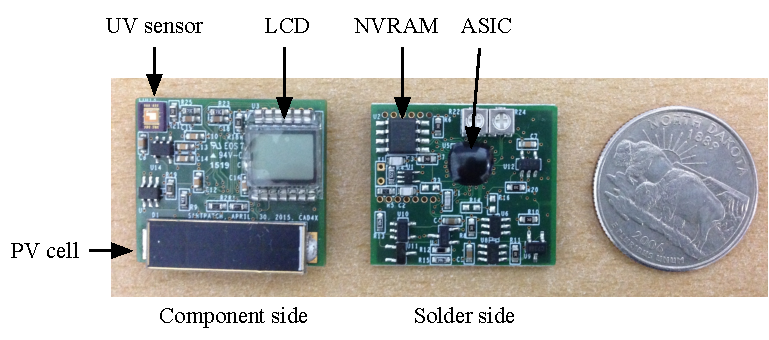
\includegraphics[width=1.0\hsize]{Figures/prototype.pdf}
\caption{A prototype of SmartPatch.}
\label{fig:prototype}
\end{figure}

Fig.~\ref{fig:prototype} shows the SmartPatch prototype implemented on a 23 mm $\times$ 22 mm board.
A custom LCD display, a PV cell and a UV sensor are on the component side of the board while the ASIC is on the solder side of the board as a chip on a board (COB) package with an NVRAM.
We add several discrete components on the both sides of the circuit board only for the debugging purpose for this version of prototype.
Table~\ref{table:prototype_summary} summarizes the implementation details of SmartPatch prototype.

\begin{table}
\centering
\caption{Summary of SmartPatch prototype.}
\label{table:prototype_summary}
\begin{tabular}{|c|c|}  \hline
Parameters			&Values	\\ \hline \hline
Size					&23 mm by 22 mm  \\ \hline
\multirow{2}{*}{Display information}	&Current UV index with one 7-segment and\\
					&remaining UV exposure time with four bars \\ \hline
User configuration		&2 skin types and use of a sunscreen (SPF 15) \\ \hline
\multirow{2}{*}{User interface}	&Reset and mode change  \\
					&by the switch-less user interface \\ \hline
Data preservation when 	&Backup and restore processes  \\
power is not enough	&with an NVRAM \\ \hline
\end{tabular}
\end{table}

Finally, we measure the power consumption of the prototype including the ASIC.
Table~\ref{table:power_summary} summarizes the power consumption of each component.
The ASIC itself consumes 1.6 mW while the other peripherals consume 6.4 mW.
In total, the prototype consumes 8 mW, which is low enough to use a small size PV cell (22 mm by 7 mm, 12.92 mW@$V_{MPP}$-3.4 V.)
%A production-level implementation with a lower-power technology and a custom electronic ink display will make the power consumption several times lower.
%
The final implementation will have a single chip ASIC including the NVRAM, an e-ink display and the optimal-size of PV cell on a flexible PCB. This is being lead by a company through technology transfer.

\begin{table}
\centering
\caption{Power consumption of SmartPatch prototype.}
\label{table:power_summary}
\begin{tabular}{|c|c|c|}  \hline
Segment 			&Components					&Power (mW)	\\ \hline \hline
3.3 V for PMU		&Clock and IO pads			&1.9	\\ \hline
1.2 V for PMU 		&Digital and analog modules		&\multirow{2}{*}{1.6}		\\
and UV meter 	&in the ASIC chip 				&\\ \hline
3.3 V for peripherals & LCD, UV sensor and NVRAM	&4.5 \\ \hline

\end{tabular}
\end{table}

%\textbf{UV irradiance varies by the skin area.}
\begin{figure}
\centering
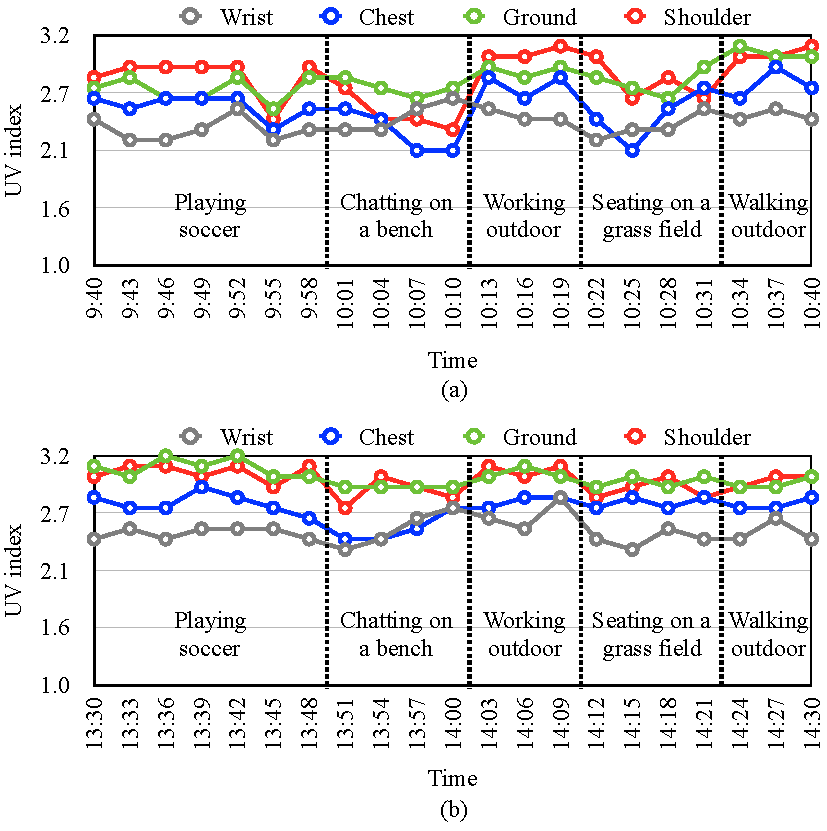
\includegraphics[width=1.0\hsize]{Figures/UV_measure.pdf}
\caption{Measurement results of UV irradiance by types of UV meters in the (a) morning and (b) afternoon.}
\label{fig:UV_measure}
\end{figure}

\textcolor{red}{To verify the functionalities and usefulness of SmartPatch, we compare the UV irradiance on various skin areas in the morning and afternoon as shown in Fig.~\ref{fig:UV_measure}. We measure the UV irradiation on the wrists, chests, shoulders, and from the ground as a reference.}
The skin area of interest in the experiment is the shoulder, and SmartPatch is attached to the shoulder skin. Other UV meters are carried or attached as designed. For instance, a watch type UV meter measures the UV irradiance on the wrist. The UV irradiance to the ground increases by the angle to the Sun that is the maximum at 1:36 pm (13:36) in the experiments.

Of course, the UV irradiance to the skin area is different by activities.
For example, playing soccer, working and walking outdoor cause high UV irradiance to the shoulder and chest as shown in Fig.~\ref{fig:UV_measure}(a).
Unfortunately, the watch type UV meter on the wrist does not reflect the UV irradiance variation on the skin area of interest, i.e., shoulders, by the activities and the angle to the Sun.
However, it is impossible to put the watch type UV meter on the shoulder.
The UV irradiance to the shoulder is sometimes even larger than the UV irradiance to the ground when the shoulder has a perpendicular angle to the Sun.

%Impact of UV measurement error on the skin damage
We observe that existing UV meters under- or overestimate the accumulation of UV irradiance.
This implies that watch type UV meters underestimate UV accumulation on the shoulder up to 16\%, which may cause 50\% more chances of erythema symptoms if UV exposure lasts until the watch type UV meters indicate the maximum exposure time is over~\cite{Harrison:Method02}.

%%%%%%%%%%%%%%%%%%%%%%%%%%%%%%%%
\section{Conclusion}
%%%%%%%%%%%%%%%%%%%%%%%%%%%%%%%%

%\textbf{SmartPatch enables range of collaborative applications.}
The storage-less and converter-less MPPT can make a UV irradiance meter small enough to be patchable.
A patchable design can make the UV irradiance measurement directly on the skin area of interest, which greatly enhances the measurement accuracy.
SmartPatch can incorporate with sunscreen lotions, tanning oils, ski goggles, hats, and so on.
SmartPatch will open more proactive UV irradiance guideline for daily life.

%%%%%%%%%%%%%%%%%%%%%%%%%%%%%%%%
%% ACKNOWLEDGMENT%%%%%%%%%%%%%%%%%%
%%%%%%%%%%%%%%%%%%%%%%%%%%%%%%%%

%\section*{Acknowledgment}
%The authors would like to thank...

%%%%%%%%%%%%%%%%%%%%%%%%%%%%%%%%
%% REFERENCE%%%%%%%%%%%%%%%%%%%%%%%
%%%%%%%%%%%%%%%%%%%%%%%%%%%%%%%%

\bibliographystyle{ieeetr}
\bibliography{smartpatch}

%%%%%%%%%%%%%%%%%%%%%%%%%%%%%%%%
%% BIOGRAPHY%%%%%%%%%%%%%%%%%%%%%%%
%%%%%%%%%%%%%%%%%%%%%%%%%%%%%%%%

%\begin{IEEEbiography}[{\includegraphics[width=1in,height=1.25in,clip,keepaspectratio]{testing.pdf}}]{Donkyu Baek}
%Biography text here.
%\end{IEEEbiography}
%
%\begin{IEEEbiography}[{\includegraphics[width=1in,height=1.25in,clip,keepaspectratio]{testing.pdf}}]{Hyung Gyu Lee}
%Biography text here.
%\end{IEEEbiography}
%
%\begin{IEEEbiography}[{\includegraphics[width=1in,height=1.25in,clip,keepaspectratio]{testing.pdf}}]{Naehyuck Chang}
%Biography text here.
%\end{IEEEbiography}

%\vfill

\end{document}


